\documentclass[11pt,a4paper]{article}
\usepackage[margin=2.5cm]{geometry}
\usepackage{amsmath,amssymb}
\usepackage{enumitem}
\usepackage{graphicx}
\usepackage{booktabs}
\usepackage[hidelinks]{hyperref}

% figures are written by the pipeline to outputs/ at the top of the repository
\graphicspath{{../outputs/}{outputs/}}

\newcommand{\given}{\,|\,}
\newcommand{\bin}{\operatorname{binomial}}
\newcommand{\pois}{\operatorname{Poisson}}
\newcommand{\Emax}{E_{\max}}
\newcommand{\Imax}{I_{\max}}
\newcommand{\Xmax}{X_{\max}}
\newcommand{\Tb}{\mathcal{T}_b}

\title{Allowing sporadic downward revisions of reported case counts\\
\large An extension of the renewal-equation reporting-delay model}
\author{}
\date{\today}

\begin{document}
\maketitle

\section{Motivation}

The model of Bajaj, Thompson and Lambert \cite{bajaj2025} assumes that the
reported count of cases with symptom onset on day $t$, when viewed from a later
day $t'$, satisfies $C(t\given t')\le I(t)$ and can only increase as $t'$
increases. Both properties follow from equation (2.2) of that paper,
\begin{equation}\label{eq:original}
C(t\given t'') - C(t\given t') \sim
\bin\bigl(I(t) - C(t\given t'),\; p_\theta(t, t''-t'\given t')\bigr),
\qquad t''>t'.
\end{equation}
In practice, counts are occasionally revised downwards, for example when a
false positive or a duplicate is removed or when a case is reassigned to a
different onset day. Here we extend the model so that such revisions have
non-zero probability, while recovering the original model as a special case.
Notation follows \cite{bajaj2025}; new symbols are introduced explicitly.

\section{Notation}

\begin{itemize}[itemsep=2pt]
\item $t=1,\dots,T$ indexes onset days.
\item $t_0<t_1<\dots<t_J$ are the times at which the count for onset day $t$
is observed. All satisfy $t_j\ge t$, and they may differ between onset days.
\item $C(t\given t_j)$ is the reported count for onset day $t$ as seen at time
$t_j$ (data).
\item $I(t)$ is the true count of cases with onset on day $t$ (latent).
\item $S_\theta(t\given t')$ is the survival function of the reporting delay
distribution with parameters $\theta$, and
$p_\theta(t,t''-t'\given t')=\bigl[S_\theta(t\given t')-S_\theta(t\given t'')\bigr]/S_\theta(t\given t')$.
\end{itemize}
As in \cite{bajaj2025}, the first observation $C(t\given t_0)$ is conditioned
on, and the likelihood is built from changes between successive observations.

\section{Model}

\subsection{Latent decomposition}

For each onset day $t$ and observation time $t_j$ we write
\begin{equation}\label{eq:decomp}
C(t\given t_j) = D(t\given t_j) + E(t\given t_j),
\end{equation}
where $D(t\given t_j)$ is the number of records held at $t_j$ for onset day $t$
that are genuine cases with onset on day $t$, and $E(t\given t_j)$ is the number
of records held at $t_j$ for onset day $t$ that are erroneous and have not yet
been withdrawn. Neither is observed.

\subsection{Increments}

Two new parameters are introduced: $\eta\ge 0$, the expected number of
erroneous records entering per genuine report, and $\rho\in(0,1)$, the daily
probability that an erroneous record is withdrawn. For onset day $t$ and the
interval $(t_{j-1},t_j]$, $j=1,\dots,J$, define
\begin{align}
\Delta C_j(t) &:= C(t\given t_j) - C(t\given t_{j-1}), \\
p_j(t) &:= p_\theta(t,\, t_j-t_{j-1}\given t_{j-1}), \\
\lambda_j(t) &:= \eta\, I(t)\,\bigl[S_\theta(t\given t_{j-1}) - S_\theta(t\given t_j)\bigr], \\
r_j &:= 1-(1-\rho)^{\,t_j-t_{j-1}}.
\end{align}
Note that $\Delta C_j(t)$ may now be negative. Within the interval, three
independent increments occur, all pertaining to onset day $t$:
\begin{align}
d_j(t) &\sim \bin\bigl(I(t) - D(t\given t_{j-1}),\; p_j(t)\bigr)
  && \text{genuine cases newly reported,} \label{eq:d}\\
n_j(t) &\sim \pois\bigl(\lambda_j(t)\bigr)
  && \text{erroneous records newly entered,} \label{eq:n}\\
m_j(t) &\sim \bin\bigl(E(t\given t_{j-1}),\; r_j\bigr)
  && \text{erroneous records withdrawn,} \label{eq:m}
\end{align}
so that
\begin{align}
D(t\given t_j) &= D(t\given t_{j-1}) + d_j(t), \\
E(t\given t_j) &= E(t\given t_{j-1}) + n_j(t) - m_j(t), \\
\Delta C_j(t) &= d_j(t) + n_j(t) - m_j(t). \label{eq:deltaC}
\end{align}

\paragraph{Conventions.}
\begin{enumerate}[label=(\roman*),itemsep=2pt]
\item Only erroneous records already present at $t_{j-1}$ can be withdrawn in
$(t_{j-1},t_j]$; a record cannot enter and be withdrawn within the same
interval.
\item Conditional on $\{I(t)\}_{t=1}^T$, $\theta$, $\eta$ and $\rho$,
increments are independent across onset days.
\item If the first observation is made on the onset day itself, $t_0=t$, then
$E(t\given t_0)=0$ and $D(t\given t_0)=C(t\given t_0)$. Otherwise, erroneous
records are assumed to have been entered and withdrawn on each of the
unobserved days $t+1,\dots,t_0$ according to \eqref{eq:n} and \eqref{eq:m}.
Since entries are Poisson and each record is withdrawn independently, it
follows that
\begin{equation}\label{eq:initialE}
E(t\given t_0)\sim\pois\bigl(\nu_0(t)\bigr),\qquad
\nu_0(t) := \eta\,I(t)\sum_{k=t+1}^{t_0}
\bigl[S_\theta(t\given k-1)-S_\theta(t\given k)\bigr](1-\rho)^{\,t_0-k},
\end{equation}
and, independently, that
\begin{equation}\label{eq:initialD}
D(t\given t_0)\sim\bin\bigl(I(t),\;p_\theta(t,\,t_0-t\given t)\bigr).
\end{equation}
\end{enumerate}

\paragraph{Properties.}
Equation \eqref{eq:d} is equation \eqref{eq:original} applied to $D$ rather
than $C$, so $D(t\given t_j)\le I(t)$ and $D$ is non-decreasing in $t_j$,
whereas $C(t\given t_j)$ may exceed $I(t)$ and may decrease. Setting $\eta=0$
gives $E\equiv 0$ and $C\equiv D$, which recovers the original model. Because
erroneous records are eventually withdrawn, $E(t\given t')\to 0$ as
$t'\to\infty$, and the identity $I(t)=C(t\given\infty)$ is retained. The mean
$\lambda_j(t)$ is $\eta$ times the expected number of genuine cases with onset
on day $t$ that are reported in $(t_{j-1},t_j]$, so erroneous records
concentrate shortly after onset and tail off as the delay distribution does.

\section{Likelihood}

Since $E(t\given t_j)$ is unobserved, we sum over it. Downward revisions are
assumed sporadic, so $E$ is truncated at a small value $\Emax$. For
$e=0,\dots,\Emax$ define the forward probabilities
\begin{equation}
\alpha_j(e;t) := P\bigl(C(t\given t_1),\dots,C(t\given t_j),\; E(t\given t_j)=e
\;\big|\; I(t),\, C(t\given t_0),\, \theta,\eta,\rho\bigr).
\end{equation}
For $j=0$ this is the distribution of $E(t\given t_0)$ given the first
observation. If $t_0=t$ then $\alpha_0(e;t)=\mathbf{1}\{e=0\}$; otherwise, from
\eqref{eq:initialE} and \eqref{eq:initialD},
\begin{equation}\label{eq:alpha0}
\alpha_0(e;t)\propto\pois\bigl(e\given\nu_0(t)\bigr)\,
\bin\bigl(C(t\given t_0)-e \given I(t),\;p_\theta(t,\,t_0-t\given t)\bigr),
\end{equation}
normalised so that $\sum_{e=0}^{\Emax}\alpha_0(e;t)=1$. For $j=1,\dots,J$,
\begin{equation}\label{eq:forward}
\begin{aligned}
\alpha_j(e;t) = \sum_{e'=0}^{\Emax} \alpha_{j-1}(e';t) \sum_{m=0}^{e'}
\;&\bin\bigl(m \given e',\, r_j\bigr) \\
\times\;&\pois\bigl(e-e'+m \given \lambda_j(t)\bigr) \\
\times\;&\bin\bigl(\Delta C_j(t)-(e-e') \given I(t)-C(t\given t_{j-1})+e',\; p_j(t)\bigr),
\end{aligned}
\end{equation}
where $\operatorname{dist}(x\given\phi)$ denotes the probability mass function
of $\operatorname{dist}$ evaluated at $x$. In the summand, with
$E(t\given t_{j-1})=e'$ and $E(t\given t_j)=e$: $m$ is $m_j(t)$; $e-e'+m$ is
$n_j(t)$; $\Delta C_j(t)-(e-e')$ is $d_j(t)$, by \eqref{eq:deltaC}; and
$I(t)-C(t\given t_{j-1})+e'$ is $I(t)-D(t\given t_{j-1})$, by \eqref{eq:decomp}.
Any term involving a negative count, or a binomial count exceeding its size,
has probability zero. The likelihood contribution of onset day $t$ is
\begin{equation}\label{eq:lik}
L_t\bigl(I(t);\theta,\eta,\rho\bigr) := \sum_{e=0}^{\Emax}\alpha_J(e;t),
\end{equation}
at a cost of $O(J\,\Emax^3)$ per value of $I(t)$. The likelihood is zero for
every value of $I(t)$ unless the reported count never falls by more than $\Emax$
from any earlier count, that is unless
\begin{equation}\label{eq:feasible}
\max_{j<k}\bigl[C(t\given t_j)-C(t\given t_k)\bigr]\le\Emax ,
\end{equation}
and, when $t_0=t$, unless $C(t\given t_j)\ge C(t\given t_0)$ for all $j$. When
$t_0>t$ the reported count may fall below the count first reported, since some
of the records present at $t_0$ may be erroneous.

\section{Changes to the sampling algorithm}

We describe the changes to the Poisson model of \cite{bajaj2025}; the
unrestricted model is modified analogously.

\paragraph{Sampling $R_t$.} Equation (2.4) of \cite{bajaj2025} is unchanged,
since it depends on the data only through $\{I(t)\}$.

\paragraph{Sampling the true case counts.} The product of binomial terms in
equation (2.6) of \cite{bajaj2025} is replaced by \eqref{eq:lik}. For
$I(t)\in\{0,1,\dots,\Imax\}$,
\begin{equation}
\begin{aligned}
q\bigl(I(t)\bigr) ={}& L_t\bigl(I(t);\theta,\eta,\rho\bigr)
\times \pois\Bigl(I(t)\,\Big|\, R_{i[t]}\sum_{s=1}^{t-1}\omega_s I(t-s)\Bigr) \\
&\times \prod_{\tau=t+1}^{T}\pois\Bigl(I(\tau)\,\Big|\, R_{i[\tau]}\sum_{s=1}^{\tau-1}\omega_s I(\tau-s)\Bigr).
\end{aligned}
\end{equation}
The lower bound $I(t)\ge C(t\given t_J)$ in equation (2.5) of \cite{bajaj2025}
is removed; values of $I(t)$ that are too small to be consistent with the data
receive zero probability through \eqref{eq:forward}. In particular
$I(t)\ge\max_j C(t\given t_j)-\Emax$. The update remains a draw
from a one-dimensional discrete distribution.

\paragraph{Sampling the reporting parameters.} Equation (2.7) of
\cite{bajaj2025} becomes
\begin{equation}\label{eq:theta}
p\bigl(\theta \,\big|\, \eta,\rho,\{I(t)\}_{t=1}^{T},\{C(t\given t_j)\}\bigr)
\propto p(\theta)\prod_{t=1}^{T}L_t\bigl(I(t);\theta,\eta,\rho\bigr),
\end{equation}
which is sampled by random-walk Metropolis as before, holding $\eta$ and $\rho$
fixed.

\paragraph{Sampling the revision parameters.} This is an additional step, which
follows the update of $\theta$. The conditional posterior is
\begin{equation}\label{eq:revision}
p\bigl(\eta,\rho \,\big|\, \theta,\{I(t)\}_{t=1}^{T},\{C(t\given t_j)\}\bigr)
\propto p(\eta)\,p(\rho)\prod_{t=1}^{T}L_t\bigl(I(t);\theta,\eta,\rho\bigr).
\end{equation}
Because both parameters are bounded and $\eta$ is expected to lie close to
zero, proposals are made on a transformed scale,
\begin{equation}
\log\eta' \sim \mathcal{N}\bigl(\log\eta,\,\sigma_\eta^2\bigr),
\qquad
\operatorname{logit}\rho' \sim \mathcal{N}\bigl(\operatorname{logit}\rho,\,\sigma_\rho^2\bigr),
\end{equation}
and the pair $(\eta',\rho')$ is accepted with probability $\min(1,r)$, where
\begin{equation}
r = \frac{p(\eta')\,p(\rho')\prod_{t=1}^{T}L_t\bigl(I(t);\theta,\eta',\rho'\bigr)}
         {p(\eta)\,p(\rho)\prod_{t=1}^{T}L_t\bigl(I(t);\theta,\eta,\rho\bigr)}
    \times\frac{\eta'\,\rho'\,(1-\rho')}{\eta\,\rho\,(1-\rho)} ,
\end{equation}
the second factor being the Jacobian of the transformation. Setting
$\sigma_\rho=0$ holds $\rho$ fixed at its initial value. We assume a gamma prior
for $\eta$ and a beta prior for $\rho$.

\section{Remarks}

\begin{itemize}[itemsep=2pt]
\item \emph{Identifiability.} The parameters $\eta$ and $\rho$ are informed
only by the rare intervals in which $\Delta C_j(t)<0$. An erroneous record not
withdrawn by $t_J$ is indistinguishable from a genuine case. Informative priors
concentrated near zero are therefore advisable (for example a gamma prior for
$\eta$ with mean and standard deviation both equal to $0.002$), and it may be
preferable to fix $\rho$.
\item \emph{Nowcasts.} For recent onset days some of $C(t\given t_J)$ may be
erroneous, so the posterior for $I(t)$ is shifted slightly downwards and
widened relative to the original model.
\item \emph{Reassigned onset days.} A case moved from onset day $t$ to onset
day $t^*$ is represented marginally, as an erroneous record on day $t$ and a
late genuine report on day $t^*$. Modelling the two jointly would couple onset
days and require block updates of $\bigl(I(t),I(t^*)\bigr)$.
\item \emph{Truncation.} $\Emax$ should be chosen so that the posterior
probability of $E(t\given t_j)=\Emax$ is negligible; this can be checked from
the forward probabilities. By \eqref{eq:feasible} it must be at least as large
as the largest fall in reported cases seen in the data, and should exceed it.
\end{itemize}

\section{Implementation}\label{sec:implementation}

The model is implemented in version 2.0 of the \texttt{incidenceinflation} R
package. Supplying initial values of $(\eta,\rho)$ to the sampler switches the
extension on; otherwise the original model is used. The following points
concern the implementation rather than the model.

\begin{itemize}[itemsep=2pt]
\item \emph{Later onset days.} Version 2.0 includes the product over later
onset days, $\tau>t$, when sampling $I(t)$, as in equation (2.6) of
\cite{bajaj2025}; earlier versions of the package conditioned only on earlier
onset days. The product is taken over at most the next 40 onset days by
default.
\item \emph{Survival function.} As in earlier versions, the survival function
is evaluated at the end of each reporting day:
$S_\theta(t\given t')=1-\operatorname{CDF}_\theta(t'+\tfrac12-t)$.
\item \emph{Onset days with complete reporting.} Onset days old enough that
reporting is deemed complete are not sampled. Their true counts are fixed at
the latest reported count, $I(t)=C(t\given t_J)$; without downward revisions
this equals the largest reported count, which earlier versions used. If $\rho$
is small, some of the records counted in $C(t\given t_J)$ may still be
erroneous, which this ignores.
\item \emph{Checks on the data.} Before sampling, the package checks
\eqref{eq:feasible} and, for onset days first observed on the onset day itself,
that the reported count never falls below the count first reported. It stops
with an error if either is violated for any onset day.
\item \emph{Negligible case counts.} Since $L_t\le 1$, the renewal terms in
$q(I(t))$ bound it from above. To reduce cost, $L_t$ is evaluated only for
values of $I(t)$ whose bound is within a factor $e^{-50}$ of $q$ at a pilot
value; the remaining values are assigned zero probability.
\item \emph{Priors.} The gamma prior for $\eta$ is specified by its mean and
standard deviation, and the beta prior for $\rho$ by its two shape parameters.
\item \emph{Optimisation.} The iterative maximisation mode of the package is
not available when downward revisions are allowed.
\item \emph{Extensions.} The extensions of \S\ref{sec:misdating} and
\S\ref{sec:batches} are both implemented and can be used separately or
together. Misdating is switched on by supplying an initial value of $\pi$ with
the shift distribution $h$, and batches by supplying the parameters of their
priors.
\item \emph{Compiled recursion.} The recursions \eqref{eq:forward} and
\eqref{eq:forwardbatch} are carried out in compiled code. A slower version of
\eqref{eq:forward} written in R is retained and used to check it.
\item \emph{Reporting parameters of neighbours.} Under misdating, the rate at
which records from a neighbouring onset day are entered is calculated using
the reporting parameters of the onset day they are entered under, which
matters only if $\theta$ differs between adjacent onset days.
\item \emph{Simulation.} Data can be simulated day by day with all three
mechanisms. Misdated cases are moved exactly in simulation, so that cases are
conserved, although the model fitted treats the two ends of a move
independently.
\end{itemize}

\paragraph{Checks.} The likelihood \eqref{eq:lik} has been verified against
direct enumeration of all paths of $\bigl(d_j(t),n_j(t),m_j(t)\bigr)$, against
the frequencies of simulated trajectories, and for summing to one over all
possible reported counts; with $\eta=0$ it reproduces the likelihood of the
original model. The starting distribution \eqref{eq:alpha0} has been verified
by checking that discarding early observations gives the same probability as
summing over them. The update of $I(t)$ has been verified against a joint
posterior obtained by exhaustive enumeration in a small example, with and
without misdating. The quantities \eqref{eq:Stilde} and \eqref{eq:lambdatilde}
have been verified against simulation. The likelihood with a batch,
\eqref{eq:likbatch}, has been verified against enumeration of all paths,
against the frequencies of simulated trajectories and by discarding early
observations. The moves which add, remove and alter batches have been verified
to reproduce the prior for $\mathcal{B}$ when the data carry no information,
and to find a simulated batch when started without one.

\section{Extension: misdated onset days}\label{sec:misdating}

\subsection{Motivation}

In the model above, every erroneous record is eventually deleted. A second
possibility is that a record is genuine but has been attributed to the wrong
onset day, and that the correction moves it to the right one. The reported
count for the wrong day then falls and, at the same reporting time, the count
for a nearby day rises. Both kinds of correction are likely to occur, and the
model here allows for both. It does so approximately: each onset day is still
treated separately, so that the fall and the rise produced by one correction
are modelled as two independent events. Cases are therefore conserved on
average but not correction by correction.

\subsection{Model for a single case}

Consider a genuine case with onset day $t$. As before, it is detected after a
delay with survival function $S_\theta$. On detection:
\begin{itemize}[itemsep=2pt]
\item with probability $1-\pi$ it is recorded under onset day $t$;
\item with probability $\pi\,h(\delta)$ it is recorded under onset day
$t+\delta$, where $h$ is a fixed probability distribution on the shifts
$\delta\in\{-H,\dots,-1,1,\dots,H\}$.
\end{itemize}
A misdated record is corrected with probability $\rho$ on each day after it is
entered, independently of all other records; on correction it is withdrawn from
onset day $t+\delta$ and recorded under onset day $t$. The new parameter is
$\pi\in[0,1)$, the probability that a case is misdated; $\pi=0$ recovers the
model of \S3. The shift distribution $h$ and its range $H$ are chosen in
advance: for example, $h$ uniform with $H=2$.

One restriction applies. A record cannot be given an onset day on or after the
day on which it is entered. A case with onset day $t$ which is detected on day
$k$ can therefore be misdated only by shifts $\delta\le k-t-1$, and is otherwise
recorded under onset day $t$. We write
\begin{equation}\label{eq:gshift}
g_t(k) := \sum_{\delta\,\le\, k-t-1} h(\delta)
\end{equation}
for the probability that a shift drawn from $h$ is possible, so that the case
is misdated with probability $\pi\,g_t(k)$. For $k\ge t+H+1$ every shift is
possible and $g_t(k)=1$.

\subsection{Consequences for a single onset day}

We now describe what this implies for the records held for onset day $t$,
treating it separately from the other onset days. Three things change.

\paragraph{Erroneous records have two sources.} The erroneous records for onset
day $t$ are now of two kinds: spurious records, which will be deleted, as in
\S3; and misdated records, which belong to cases with onset on a nearby day.
A case with onset day $t-\delta$ which is detected in $(t_{j-1},t_j]$ is
recorded under $t$ with probability $\pi\,h(\delta)$. We take the number of
erroneous records newly entered for onset day $t$ to be
$n_j(t)\sim\pois\bigl(\tilde\lambda_j(t)\bigr)$, replacing \eqref{eq:n}, where
\begin{equation}\label{eq:lambdatilde}
\tilde\lambda_j(t) := \lambda_j(t)
+ \pi\sum_{\substack{\delta=-H\\ \delta\neq 0}}^{H} h(\delta)\,I(t-\delta)\,
\bigl[S_\theta(t-\delta\given t_{j-1})-S_\theta(t-\delta\given t_j)\bigr],
\end{equation}
with $I(s):=0$ for onset days $s$ outside the period studied and
$S_\theta(s\given t'):=1$ for $t'<s$, since a case cannot be detected before
its onset. The first term is the rate of spurious records and the second the
rate of misdated ones.

\paragraph{Both kinds are withdrawn in the same way.} A spurious record is
deleted, and a misdated record is corrected, with the same daily probability
$\rho$. While they are held under onset day $t$ the two kinds therefore behave
identically, and a single count $E(t\given t_j)$ of erroneous records still
suffices; \eqref{eq:m} is unchanged. Reported counts alone could not in any case
distinguish a rate of deletion from a rate of correction.

\paragraph{Genuine reports can arrive late.} A case with onset day $t$ which is
misdated is recorded under $t$ only when it is corrected. Let $V$ be the number
of days from entry to correction, with $P(V=v)=\rho(1-\rho)^{v-1}$ for
$v=1,2,\dots$ The probability that a case with onset day $t$ has not yet been
recorded under $t$ by day $t'$ is then
\begin{equation}\label{eq:Stilde}
\tilde S_\theta(t\given t') := S_\theta(t\given t')
+ \pi\sum_{k=t+1}^{t'}g_t(k)\,\bigl[S_\theta(t\given k-1)-S_\theta(t\given k)\bigr](1-\rho)^{\,t'-k}.
\end{equation}
The first term is the probability that the case is undetected. In the second,
each summand is the probability that the case was detected on day $k$, that a
shift was possible and, if misdated, that it has not been corrected by day
$t'$. Genuine cases are newly recorded
under onset day $t$ according to \eqref{eq:d} with $p_j(t)$ replaced by
\begin{equation}\label{eq:ptilde}
\tilde p_j(t) := \frac{\tilde S_\theta(t\given t_{j-1})-\tilde S_\theta(t\given t_j)}
{\tilde S_\theta(t\given t_{j-1})}.
\end{equation}
Here $D(t\given t_j)$ is the number of genuine cases recorded under onset day
$t$, so that a case with onset day $t$ which is currently misdated counts among
the $I(t)-D(t\given t_j)$ yet to be recorded. Since every misdated record is
eventually corrected, the identity $I(t)=C(t\given\infty)$ is retained.

\paragraph{First observation.} The starting distribution \eqref{eq:alpha0} is
obtained as before, with $\lambda$ replaced by $\tilde\lambda$ in
$\nu_0(t)$ and $S_\theta$ replaced by $\tilde S_\theta$ in
$p_\theta(t,t_0-t\given t)$.

\subsection{Likelihood and sampling}

The recursion \eqref{eq:forward} is unchanged in form, with $\tilde\lambda_j(t)$
and $\tilde p_j(t)$ in place of $\lambda_j(t)$ and $p_j(t)$. Through
\eqref{eq:lambdatilde}, the likelihood contribution of onset day $t$ now
depends on the true counts of its neighbours as well as its own:
\begin{equation}
L_t = L_t\bigl(I(t-H),\dots,I(t+H);\,\theta,\eta,\pi,\rho\bigr).
\end{equation}
The sampling steps change as follows.
\begin{itemize}[itemsep=2pt]
\item \emph{True case counts.} $I(t)$ appears in the likelihood contributions
of onset days $t-H,\dots,t+H$, so that
\begin{equation}
\begin{aligned}
q\bigl(I(t)\bigr) ={}& \Biggl[\,\prod_{s=t-H}^{t+H}L_s\Biggr]
\times \pois\Bigl(I(t)\,\Big|\, R_{i[t]}\sum_{s=1}^{t-1}\omega_s I(t-s)\Bigr) \\
&\times \prod_{\tau=t+1}^{T}\pois\Bigl(I(\tau)\,\Big|\, R_{i[\tau]}\sum_{s=1}^{\tau-1}\omega_s I(\tau-s)\Bigr),
\end{aligned}
\end{equation}
where the first product is over those onset days which lie within the period
studied. The update remains a draw from a one-dimensional discrete
distribution, at about $2H+1$ times the cost.
\item \emph{Reporting parameters.} As in \eqref{eq:theta}, with the new $L_t$.
\item \emph{Revision parameters.} $\pi$ joins $\eta$ and $\rho$ in
\eqref{eq:revision}, with a beta prior and proposals made for
$\operatorname{logit}\pi$.
\item \emph{$R_t$.} Unchanged.
\end{itemize}

\subsection{Remarks}

\begin{itemize}[itemsep=2pt]
\item \emph{What is approximate.} A correction is one event: a record leaves
one onset day and joins another at the same reporting time. Here the departure
is a withdrawal on one onset day and the arrival is a late genuine report on
another, and the two are treated as independent. The expected numbers agree,
so cases are conserved on average, but the information in a fall and a rise
occurring together on nearby onset days is not used. Taking $n_j(t)$ to be
Poisson and independent of the genuine reports is part of the same
approximation.
\item \emph{Late upward revisions.} Without misdating, a rise in the reported
count long after onset must be explained by the tail of the reporting delay
distribution, which distorts the estimate of $\theta$. Under
\eqref{eq:Stilde} such rises are instead attributed to corrections, whose
timing is governed by $\rho$.
\item \emph{Deletion and misdating are hard to separate.} Both $\eta$ and $\pi$
produce falls in the reported count. They differ only in that misdating also
produces late rises on nearby onset days, and in the dependence of
\eqref{eq:lambdatilde} on neighbouring counts. The total rate at which
erroneous records are entered should be better determined than its division
between the two, which will depend on the priors.
\item \emph{A simplification.} If the true counts vary slowly from one onset
day to the next, the second term of \eqref{eq:lambdatilde} is approximately
$\pi\,I(t)\,[S_\theta(t\given t_{j-1})-S_\theta(t\given t_j)]$. Then
$\tilde\lambda_j(t)$ has the form of $\lambda_j(t)$ with $\eta+\pi$ in place of
$\eta$, each $L_t$ depends only on $I(t)$, and the only change to the model of
\S3 is \eqref{eq:Stilde}. This is not appropriate when counts differ sharply
between adjacent onset days.
\item \emph{Batches.} The extension of \S\ref{sec:batches} is unaffected in
form: it uses $\tilde\lambda_j(t)$ and $\tilde p_j(t)$ in place of
$\lambda_j(t)$ and $p_j(t)$.
\end{itemize}

\section{Extension: corrections made in batches}\label{sec:batches}

\subsection{Motivation}

The model above withdraws each erroneous record independently, with a constant
daily probability $\rho$. It is therefore suited to small revisions scattered
across onset days and reporting times. In practice, records are also corrected
in batches: for example, all cases from a particular place, or all cases
confirmed in a particular run of laboratory tests, come to be regarded as
suspect and are removed together. Such a correction has three features which
the model above cannot reproduce: the fall in reported cases is large; it
happens at a single reporting time, possibly long after onset; and it affects
several adjacent onset days at once.

We therefore suppose that erroneous records can share a \emph{mark}, which
identifies the batch they belong to, and that it is the mark which is detected:
when it is, every record carrying it is withdrawn. The erroneous records of
\S3 are the special case in which every batch consists of a single record.

\subsection{Batches}

There are $K$ batches, indexed by $b=1,\dots,K$, where $K$ is unknown. Batch
$b$ is described by four quantities.
\begin{itemize}[itemsep=2pt]
\item Its \emph{footprint}, $\Tb=\{a_b,a_b+1,\dots,a_b+w_b-1\}$: a set of $w_b$
consecutive onset days, starting at onset day $a_b$, to which its records are
attributed.
\item Its \emph{intensity}, $\phi_b>0$: the expected number of its records
entered per genuine case reported, for each onset day in its footprint.
\item Its \emph{detection time}, $\tau_b$: the day on which its mark is
detected.
\end{itemize}
Footprints do not overlap, so that each onset day $t$ belongs to the footprint
of at most one batch, which we write $b(t)$ when it exists.

\paragraph{Priors.} Batches are rare, and the prior for their footprints is
constructed so that they cannot overlap. Consider the onset days in order,
$t=1,\dots,T$. If onset day $t$ lies in the footprint of a batch which started
on an earlier day, no batch starts on it. Otherwise, a batch starts on it with
probability $\beta\ll 1$, in which case its width is drawn as
$w_b-1\sim\pois(\zeta)$. At most one batch can therefore start on any onset
day, and no batch can start inside the footprint of another. Writing $F$ for
the number of onset days which lie in no footprint, the prior probability of
the footprints is
\begin{equation}\label{eq:footprintprior}
p\bigl(\{(a_b,w_b)\}_{b=1}^{K}\bigr)
= \beta^{K}\,(1-\beta)^{F}\prod_{b=1}^{K}\pois\bigl(w_b-1\given\zeta\bigr).
\end{equation}
A footprint may extend beyond the last onset day $T$, and we ignore batches
which started before the first onset day. Intensities are independent across
batches, with $\phi_b$ having a gamma prior. Each batch is
detected with the same probability $\rho_B$ on each day after its footprint
starts, whatever its size:
\begin{equation}\label{eq:detection}
P(\tau_b=s) = \rho_B\,(1-\rho_B)^{\,s-a_b-1},\qquad s=a_b+1,a_b+2,\dots
\end{equation}
Since a batch is eventually detected with probability one, the identity
$I(t)=C(t\given\infty)$ is retained.

\subsection{Reported counts}

Let $X(t\given t_j)$ be the number of records of batch $b(t)$ held at $t_j$ for
onset day $t$, with $X(t\given t_j)\equiv 0$ if $t$ is in no footprint. The
decomposition \eqref{eq:decomp} becomes
\begin{equation}\label{eq:decompbatch}
C(t\given t_j) = D(t\given t_j) + E(t\given t_j) + X(t\given t_j),
\end{equation}
where $D$ and $E$ evolve exactly as in \S3. For an onset day $t\in\Tb$, let
\begin{equation}
j_b(t) := \min\{\,j : t_j\ge\tau_b\,\}
\end{equation}
index the first observation of onset day $t$ made at or after the detection
time; if there is none, the batch is still undetected at $t_J$ and we set
$j_b(t)=\infty$. Then, for $j=1,\dots,J$,
\begin{align}
u_j(t) &\sim \pois\bigl(\phi_b\, I(t)\,[S_\theta(t\given t_{j-1})-S_\theta(t\given t_j)]\bigr)
 && \text{batch records newly entered, if } j<j_b(t), \label{eq:u}\\
X(t\given t_j) &=
\begin{cases}
X(t\given t_{j-1}) + u_j(t), & j<j_b(t),\\
0, & j\ge j_b(t),
\end{cases} \label{eq:X}
\end{align}
and $u_j(t)=0$ for $j\ge j_b(t)$. That is, the records of a batch enter in
proportion to genuine reports, as in \eqref{eq:n}; none of them is withdrawn
before detection; all of them are withdrawn at the first observation at or
after detection; and none enters thereafter. The change in the reported count
is
\begin{equation}\label{eq:deltaCbatch}
\Delta C_j(t) = d_j(t) + n_j(t) - m_j(t) + X(t\given t_j) - X(t\given t_{j-1}).
\end{equation}
At the detection time the last term equals $-X(t\given t_{j-1})$ for every
onset day in the footprint simultaneously, which produces the large,
coincident falls described above.

\paragraph{First observation.} If $t_0=t$ then $X(t\given t_0)=0$. If
$t<t_0<\tau_b$, the records of the batch have accumulated over the unobserved
days without withdrawal, so that, independently of $D(t\given t_0)$ and
$E(t\given t_0)$,
\begin{equation}\label{eq:initialX}
X(t\given t_0)\sim\pois\bigl(\xi_0(t)\bigr),\qquad
\xi_0(t) := \phi_b\,I(t)\,\bigl[S_\theta(t\given t)-S_\theta(t\given t_0)\bigr].
\end{equation}
If $t_0\ge\tau_b$, the batch was removed before onset day $t$ was first
observed and $X(t\given t_j)=0$ for all $j$.

\subsection{Likelihood}

Conditional on the batches, that is on
$\mathcal{B}:=\{(a_b,w_b,\phi_b,\tau_b)\}_{b=1}^{K}$, onset days remain
independent. For an onset day in no footprint, the likelihood is $L_t$ of
\eqref{eq:lik}, unchanged. For $t\in\Tb$ we sum over both hidden counts,
truncating $X$ at $\Xmax$. Define, for $e=0,\dots,\Emax$ and
$x=0,\dots,\Xmax$,
\begin{equation}
\alpha_j(e,x;t) := P\bigl(C(t\given t_1),\dots,C(t\given t_j),\;
E(t\given t_j)=e,\;X(t\given t_j)=x
\;\big|\; I(t),\, C(t\given t_0),\, \theta,\eta,\rho,\mathcal{B}\bigr).
\end{equation}
Let
\begin{equation}\label{eq:g}
\begin{aligned}
g_j(k\given e',e,x';t) := {}&
\bin\bigl(k\given I(t)-C(t\given t_{j-1})+e'+x',\;p_j(t)\bigr)\\
&\times\sum_{m=0}^{e'}\bin\bigl(m\given e',\,r_j\bigr)\,
\pois\bigl(e-e'+m\given\lambda_j(t)\bigr)
\end{aligned}
\end{equation}
be the probability that $k$ genuine cases are newly reported and that the
erroneous count moves from $e'$ to $e$ in the interval $(t_{j-1},t_j]$, given
that $E(t\given t_{j-1})=e'$ and $X(t\given t_{j-1})=x'$. Here
$I(t)-C(t\given t_{j-1})+e'+x'$ is $I(t)-D(t\given t_{j-1})$, by
\eqref{eq:decompbatch}. The recursion is as follows.
\begin{itemize}[itemsep=2pt]
\item Before detection, $j<j_b(t)$:
\begin{equation}\label{eq:forwardbatch}
\begin{aligned}
\alpha_j(e,x;t)=\sum_{e'=0}^{\Emax}\sum_{x'=0}^{x}\;&\alpha_{j-1}(e',x';t)\\
\times\;&\pois\bigl(x-x'\given\phi_b\, I(t)\,[S_\theta(t\given t_{j-1})-S_\theta(t\given t_j)]\bigr)\\
\times\;&g_j\bigl(\Delta C_j(t)-(e-e')-(x-x')\given e',e,x';t\bigr).
\end{aligned}
\end{equation}
\item At detection, $j=j_b(t)$: $\alpha_j(e,x;t)=0$ for $x>0$, and
\begin{equation}\label{eq:forwarddetect}
\alpha_j(e,0;t)=\sum_{e'=0}^{\Emax}\sum_{x'=0}^{\Xmax}\alpha_{j-1}(e',x';t)\,
g_j\bigl(\Delta C_j(t)-(e-e')+x'\given e',e,x';t\bigr).
\end{equation}
\item After detection, $j>j_b(t)$: $x=0$ and the recursion is
\eqref{eq:forward}.
\end{itemize}
The recursion starts from
$\alpha_0(e,x;t)\propto\pois(e\given\nu_0(t))\,\pois(x\given\xi_0(t))\,
\bin\bigl(C(t\given t_0)-e-x\given I(t),\,p_\theta(t,t_0-t\given t)\bigr)$,
normalised to sum to one, with the modifications for $t_0=t$ and
$t_0\ge\tau_b$ given above. The likelihood contribution of onset day $t$ is
\begin{equation}\label{eq:likbatch}
L_t\bigl(I(t);\theta,\eta,\rho,\mathcal{B}\bigr)
:=\sum_{e=0}^{\Emax}\sum_{x=0}^{\Xmax}\alpha_J(e,x;t).
\end{equation}
Terms of this sum with $x>0$ correspond to a batch which has not yet been
detected at $t_J$. The additional cost, a factor of order $\Xmax^2$, is
incurred only for onset days inside a footprint.

\subsection{Sampling}

The updates of $R_t$, $I(t)$, $\theta$ and $(\eta,\rho)$ are as before, with
\eqref{eq:likbatch} in place of \eqref{eq:lik}. There is one additional step,
which updates the batches:
\begin{equation}
p\bigl(\mathcal{B}\,\big|\,\{I(t)\},\{C(t\given t_j)\},\theta,\eta,\rho\bigr)
\propto p(\mathcal{B})\prod_{t=1}^{T}L_t\bigl(I(t);\theta,\eta,\rho,\mathcal{B}\bigr),
\end{equation}
where $p(\mathcal{B})$ is given by the priors above, including
\eqref{eq:footprintprior} and \eqref{eq:detection}. Since $K$ is unknown this requires moves which add and
remove a batch, as well as moves which change the footprint, intensity or
detection time of an existing batch. Each such move changes $L_t$ only for
onset days in the footprints concerned.

\paragraph{Adding and removing a batch.} In each iteration one move is
attempted which, with equal probability, adds a batch or removes one chosen
uniformly at random. A batch to be added has its intensity drawn from the
prior for $\phi_b$ and its footprint and detection time drawn from a
distribution $q$. With probability one half, $q$ draws from the prior: the
start $a_b$ uniformly from the $T$ onset days, $w_b-1\sim\pois(\zeta)$ and
$\tau_b$ from \eqref{eq:detection}. Otherwise, $q$ draws uniformly from a list
of \emph{candidates} found from the data in advance: reporting times at which
the reported counts for a run of adjacent onset days fall together, by a total
of at least some threshold. A proposal whose footprint overlaps that of an
existing batch is rejected. Otherwise, with $K$ batches at present and $n$
onset days in the proposed footprint, it is accepted with probability
$\min(1,r)$, where
\begin{equation}\label{eq:birth}
r = \frac{\prod_{t}L_t(\,\cdot\,;\mathcal{B}')}{\prod_{t}L_t(\,\cdot\,;\mathcal{B})}
\times
\frac{\beta\,(1-\beta)^{-n}\,\pois(w_b-1\given\zeta)\,P(\tau_b)}
     {(K+1)\,q(a_b,w_b,\tau_b)} ,
\end{equation}
the products being over the onset days in the proposed footprint. Removing a
batch is accepted with the reciprocal of this ratio, evaluated with $K$ the
number of batches remaining.

\paragraph{Altering a batch.} For each batch in turn, three proposals are made
and accepted or rejected in the usual way: to multiply $\phi_b$ by a
log-normal factor; to move $\tau_b$ by up to three days in either direction;
and to extend or shorten the footprint by one onset day at either end.

\paragraph{Hyperparameters.} With priors $\beta\sim\operatorname{beta}(a_\beta,b_\beta)$,
$\zeta\sim\operatorname{gamma}(a_\zeta,b_\zeta)$ and
$\rho_B\sim\operatorname{beta}(a_\rho,b_\rho)$, the conditional posteriors are
\begin{equation}
\begin{aligned}
\beta &\sim\operatorname{beta}(a_\beta+K,\;b_\beta+F),\\
\zeta &\sim\operatorname{gamma}\Bigl(a_\zeta+\sum_b (w_b-1),\;b_\zeta+K\Bigr),\\
\rho_B &\sim\operatorname{beta}\Bigl(a_\rho+K,\;b_\rho+\sum_b(\tau_b-a_b-1)\Bigr),
\end{aligned}
\end{equation}
from which each is drawn directly. Any of them can alternatively be held
fixed.

\paragraph{Starting values.} Sampling starts with only those candidates
without which the reported counts would be impossible: those containing a
single fall larger than $\Emax$.

Batches which have not yet been detected form part of $\mathcal{B}$. There is
no direct evidence for these, so they are sampled almost entirely from the
prior, conditional on having survived undetected.

\subsection{Remarks}

\begin{itemize}[itemsep=2pt]
\item \emph{What the data can identify.} A batch is indistinguishable from
genuine cases until it is detected. The parameters $\beta$, $\zeta$, $\rho_B$
and the prior for $\phi_b$ are therefore informed only by the batches removed
within the period observed, of which there may be very few, and will depend
strongly on their priors.
\item \emph{Nowcasts.} For recent onset days the model contributes a risk
rather than a correction: with some probability, part of the reported count
belongs to a batch not yet detected. This widens the posterior for $I(t)$ and
lowers it slightly, but cannot indicate which onset days are affected. By
contrast, explaining a large fall with the model of \S3 would require a large
$\eta$, which would lower the estimates for every recent onset day.
\item \emph{Detection per batch or per record.} An alternative to
\eqref{eq:detection} is that each record is flagged with daily probability
$\rho$ and that flagging any record exposes its batch, so that a batch holding
$N$ records is detected on a given day with probability $1-(1-\rho)^N$ and
large batches are found sooner. With one record per batch this is exactly the
model of \S3. A large batch which persists for a long time before being removed
is evidence for \eqref{eq:detection} instead.
\item \emph{Reinstated cases.} If the cases in a suspect batch are re-examined
and some are reinstated, the removal is partly temporary. Treating the whole
batch as erroneous would then understate $I(t)$.
\item \emph{Overlapping footprints.} These are excluded because the data could
rarely distinguish two batches covering the same onset days from one.
\item \emph{Marks which are observed.} If the data record the place or
laboratory for each case, as in a line list, the mark is observed directly and
the batches need not be inferred from falls in the counts.
\end{itemize}

\section{Simulation study}\label{sec:simulation}

The numbers and figures in this section and the next are produced by the
pipeline in this repository (\texttt{\_targets.R}); the tables are copied from
\texttt{outputs/results.md}.

\subsection{Design}

Data were simulated for $T=60$ onset days and observed daily up to day 60. In
all cases $R_t=1.3$ for the first 30 onset days and $0.9$ thereafter, the
serial interval had mean 5 and standard deviation 3 days, and the reporting
delay had mean 5 and standard deviation 3 days. Five regimes were considered,
which differ in how reported counts are revised (table~\ref{tab:regimes}).
Where cases are misdated, shifts of $\pm1$ day each have probability $0.35$
and shifts of $\pm2$ days each have probability $0.15$. Where there is a
batch, its footprint is onset days 28 to 34, its intensity is $\phi_b=0.25$
and it is detected on day 48. Five datasets were simulated under each regime.

\begin{table}[h]
\centering
\begin{tabular}{llllc}
\toprule
Regime & $\eta$ & $\rho$ & $\pi$ & Batch \\
\midrule
None & -- & -- & -- & no \\
Sporadic & 0.03 & 0.15 & -- & no \\
Misdating & 0.005 & 0.15 & 0.10 & no \\
Batch & 0.005 & 0.15 & -- & yes \\
Combined & 0.03 & 0.15 & 0.10 & yes \\
\bottomrule
\end{tabular}
\caption{Regimes under which data were simulated.}\label{tab:regimes}
\end{table}

Three models were fitted to each dataset.
\begin{itemize}[itemsep=2pt]
\item \emph{Original}: the model of \cite{bajaj2025}, in which reported counts
can only rise. Since it cannot be fitted to counts which fall, the reported
counts for each onset day were first replaced by their running maximum.
\item \emph{Sporadic}: the model of \S3, with $\Emax=10$.
\item \emph{Full}: the model of \S3 with the extensions of
\S\ref{sec:misdating} and \S\ref{sec:batches}, with $\Emax=10$ and $\Xmax=60$.
\end{itemize}
$R_t$ was piecewise-constant over periods of 15 onset days. Each fit was a
single chain of 700 iterations, of which the first half was discarded. Priors
were: $R_t\sim\operatorname{gamma}(1,1)$; gamma priors for the mean and
standard deviation of the reporting delay with means 5 and 3 and standard
deviations 10 and 5; a gamma prior for $\eta$ with mean and standard deviation
$0.02$; $\rho\sim\operatorname{beta}(1,4)$; $\pi\sim\operatorname{beta}(1,9)$;
and, for batches, $\beta\sim\operatorname{beta}(1,199)$, $\zeta=4$,
$\rho_B=0.05$ and a gamma prior for $\phi_b$ with mean $0.3$ and standard
deviation $0.2$.

\subsection{Results}

Table~\ref{tab:simulation} and figure~\ref{fig:simulationscores} summarise how
well each model recovered the true case counts. Figure~\ref{fig:simulationexamples}
shows the first dataset from each regime.

\begin{table}[h]
\centering
\begin{tabular}{llcccccc}
\toprule
 & & \multicolumn{3}{c}{Latest 14 onset days} & \multicolumn{2}{c}{Batch onset days} & \\
\cmidrule(lr){3-5}\cmidrule(lr){6-7}
Regime & Model & Coverage & Abs.\ error & Bias & Abs.\ error & Bias & Latest $R_t$ \\
\midrule
None & Original & 0.89 & 0.05 & $-0.01$ & & & 0.91 \\
 & Sporadic & 0.89 & 0.05 & $-0.01$ & & & 0.91 \\
 & Full & 0.89 & 0.05 & $-0.01$ & & & 0.91 \\
\addlinespace
Sporadic & Original & 0.93 & 0.06 & $0.01$ & & & 0.91 \\
 & Sporadic & 0.91 & 0.06 & $0.00$ & & & 0.91 \\
 & Full & 0.91 & 0.06 & $0.00$ & & & 0.91 \\
\addlinespace
Misdating & Original & 0.80 & 0.06 & $0.03$ & & & 0.92 \\
 & Sporadic & 0.89 & 0.06 & $0.02$ & & & 0.92 \\
 & Full & 0.93 & 0.07 & $-0.01$ & & & 0.91 \\
\addlinespace
Batch & Original & 0.90 & 0.05 & $-0.01$ & 0.26 & $0.26$ & 0.88 \\
 & Sporadic & \multicolumn{6}{c}{could not be fitted} \\
 & Full & 0.91 & 0.05 & $0.00$ & 0.00 & $0.00$ & 0.88 \\
\addlinespace
Combined & Original & 0.77 & 0.07 & $0.04$ & 0.25 & $0.25$ & 0.92 \\
 & Sporadic & \multicolumn{6}{c}{could not be fitted} \\
 & Full & 0.84 & 0.06 & $0.02$ & 0.01 & $0.00$ & 0.92 \\
\bottomrule
\end{tabular}
\caption{Performance on simulated data: means across five datasets per regime.
Coverage is that of 90\% posterior intervals. Absolute error and bias are those
of the posterior median of the case count, relative to the mean true count:
a bias of $0.03$ means that estimates were on average 3\% of the mean count too
high. The final column is the estimate of $R_t$ for the latest period, onset
days 46 to 60, for which the true value is $0.9$: the posterior median,
averaged across datasets.}
\label{tab:simulation}
\end{table}

\begin{figure}[p]
\centering
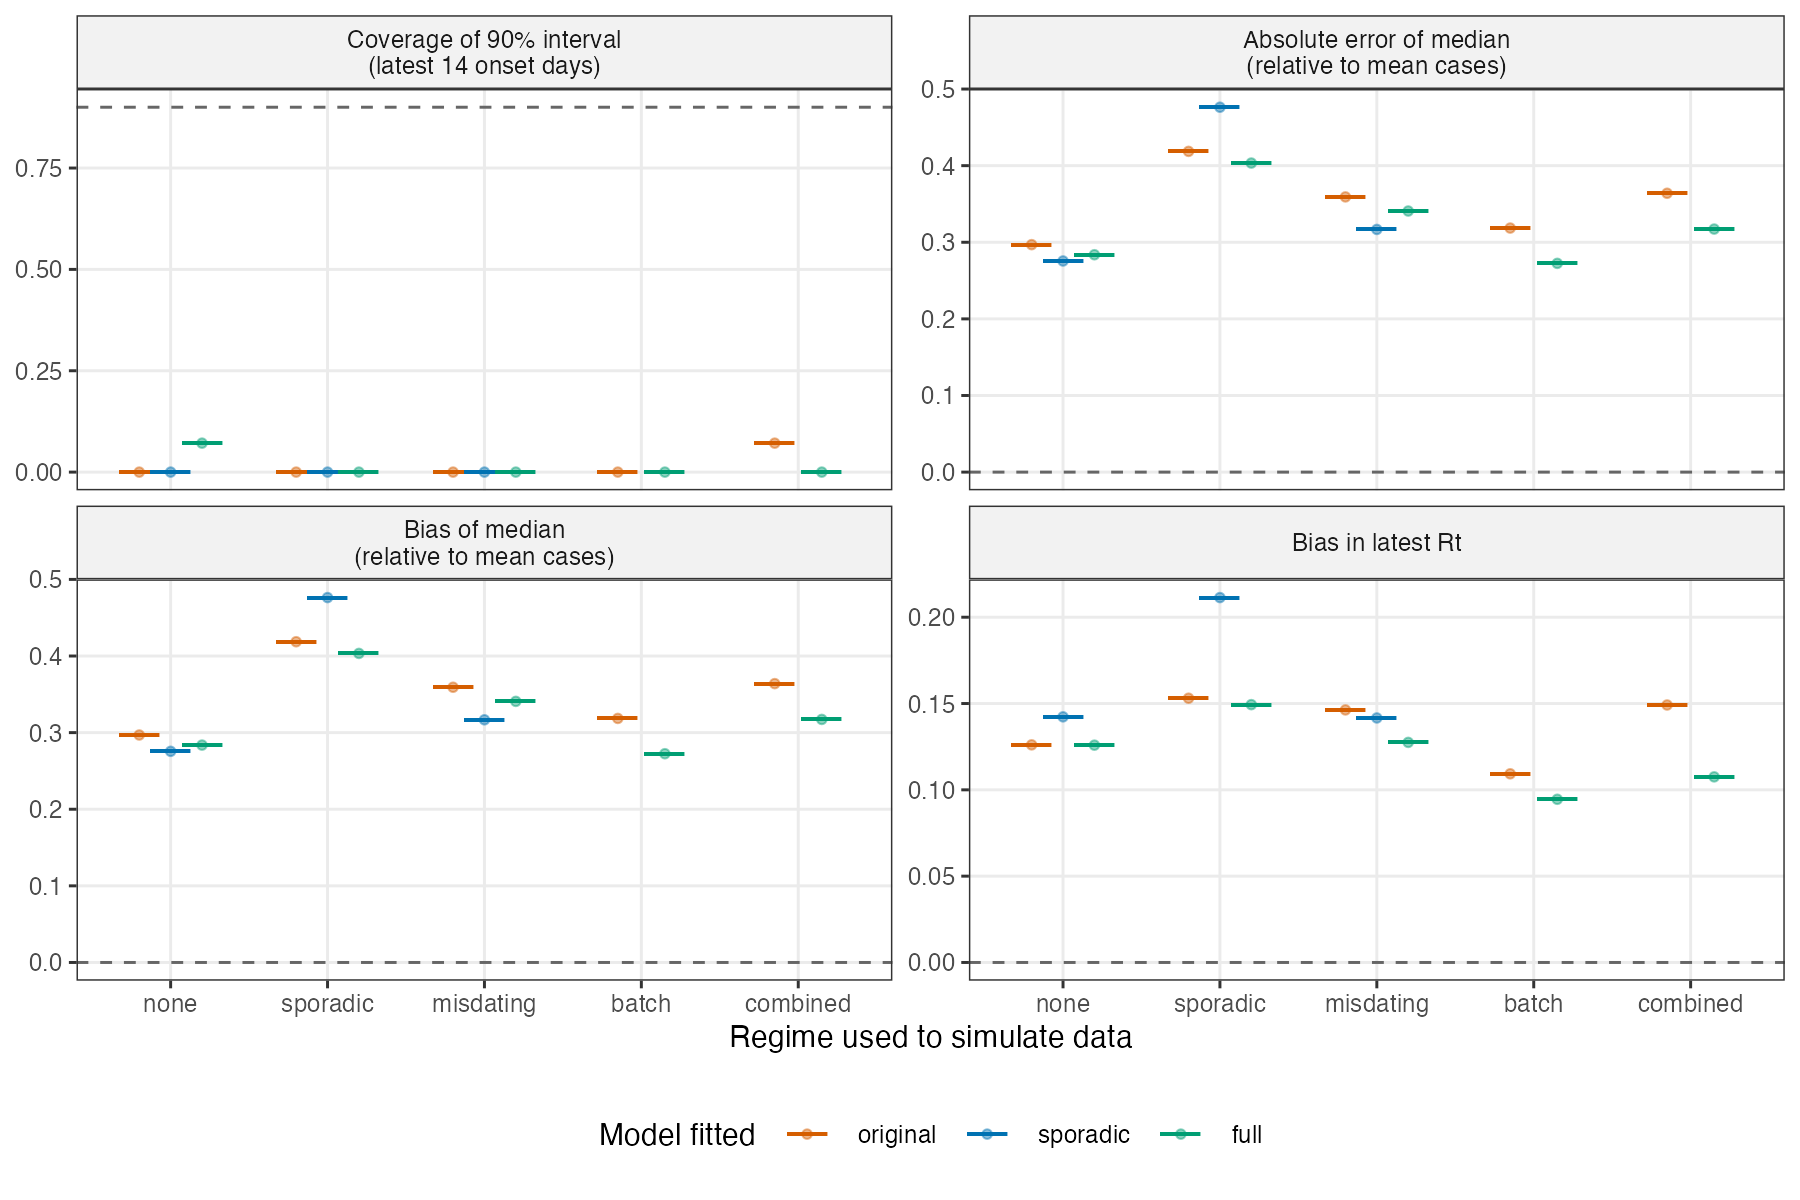
\includegraphics[width=\textwidth]{simulation_scores.png}
\caption{Performance of each model on each simulated dataset (points) and the
mean across datasets (bars), by the regime used to simulate.}
\label{fig:simulationscores}
\end{figure}

\begin{figure}[p]
\centering
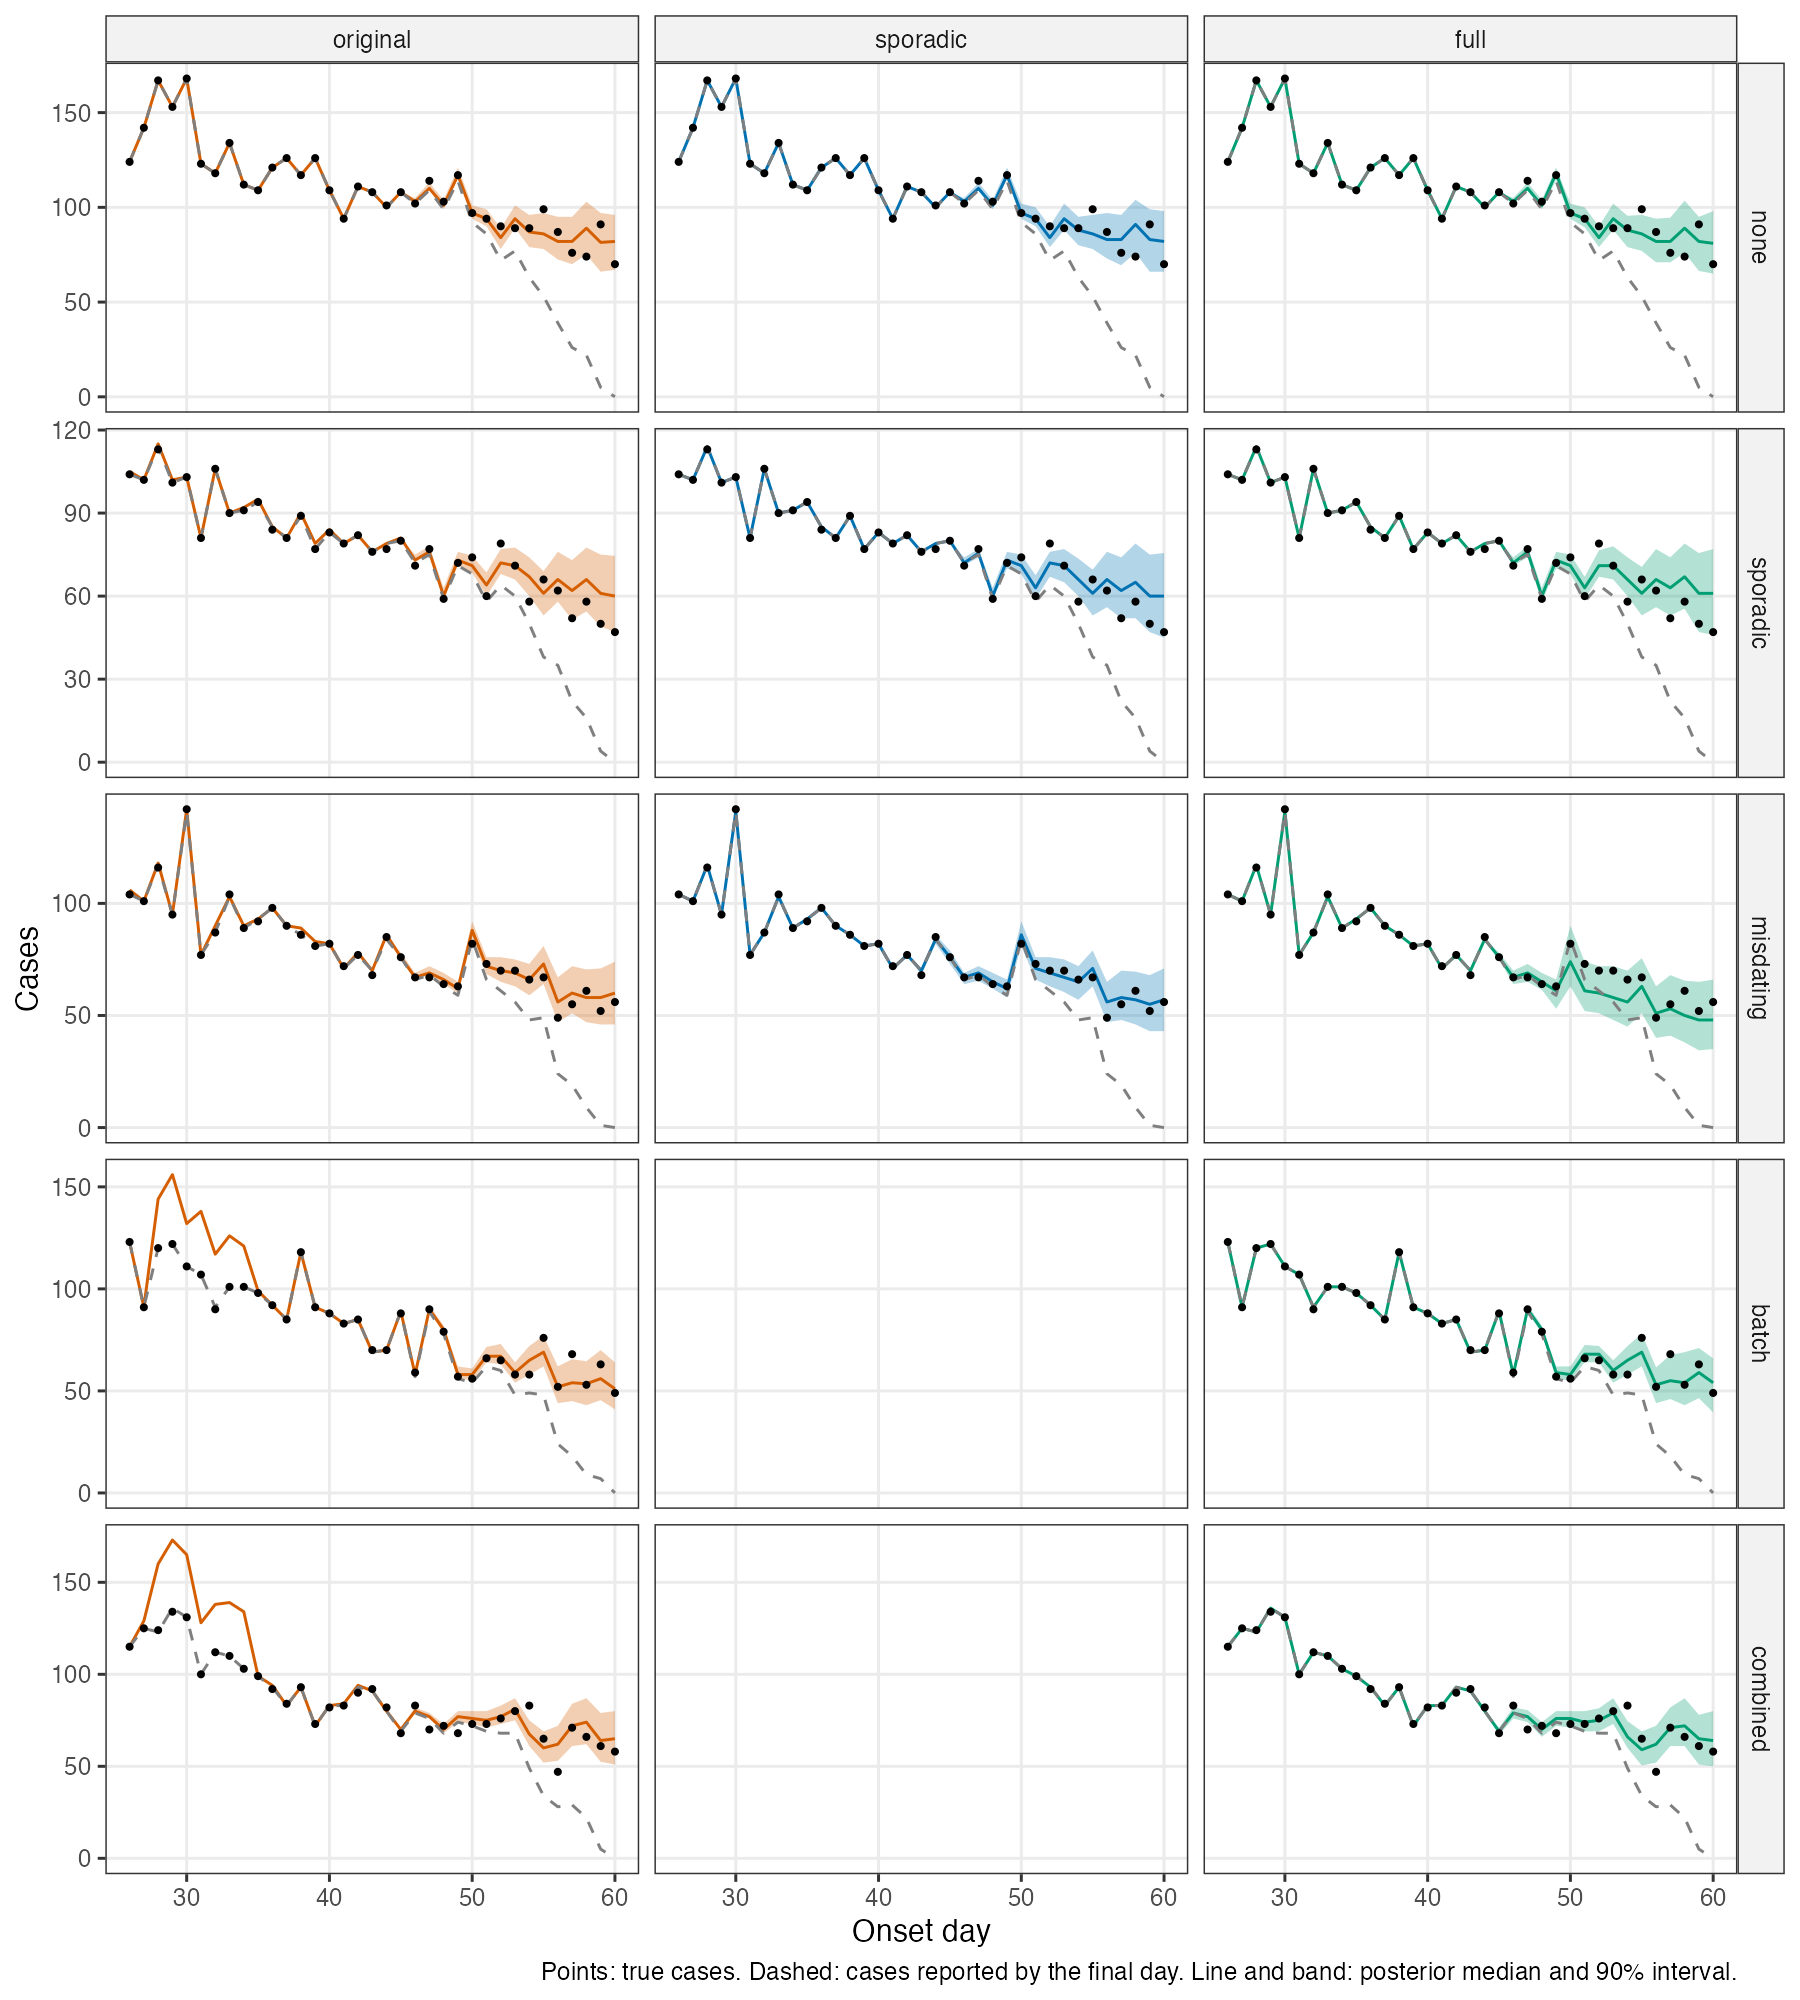
\includegraphics[width=0.95\textwidth]{simulation_examples.png}
\caption{Estimates of true case counts for the first dataset simulated under
each regime (rows), for each model (columns).}
\label{fig:simulationexamples}
\end{figure}

\begin{itemize}[itemsep=2pt]
\item \emph{No revisions.} The three models gave the same results. The full
model placed little posterior probability on there being any batch (0.05 on
average).
\item \emph{Sporadic revisions.} The three models performed equally well. The
sporadic model recovered the revision parameters (posterior medians averaging
$\eta=0.024$ and $\rho=0.15$, against true values of $0.03$ and $0.15$), but at
this rate of revision replacing counts by their running maximum served as well
for the purpose of estimating recent case counts.
\item \emph{Misdating.} The full model had the best coverage for recent onset
days (0.93, against 0.80 for the original model) and recovered the misdating
probability (posterior median averaging $0.089$, against a true value of
$0.10$). The sporadic model accounted for misdated records with a larger rate
of spurious records ($\eta=0.11$) and overestimated the mean reporting delay
(5.5 days, against a true value of 5).
\item \emph{A batch.} For the onset days in the footprint of the batch, the
original model overestimated the true counts by about a quarter, since the
running maximum retains the records of the batch. The full model identified
the batch in every dataset and recovered the true counts. The sporadic model
could not be fitted, since falls of this size are impossible under it.
\item \emph{Combined.} The full model again recovered the counts for the onset
days in the footprint, with an absolute error of under 1\%.
\end{itemize}

\paragraph{Caveats.} There are only five datasets per regime, so that
differences of a few percentage points are within noise. Each fit is a single
short chain and convergence was not assessed formally. The full model took
about half an hour per fit, against five to ten minutes for the others. Onset
days for which reporting is deemed complete are fixed at their latest reported
count (\S\ref{sec:implementation}), so their posterior intervals have zero
width; coverage is therefore not reported for the onset days in the footprint
of the batch.

\section{Application: COVID-19 in the Netherlands}\label{sec:netherlands}

\subsection{Data}

During 2020 the Dutch National Institute for Public Health and the Environment
(RIVM) published a file each day listing every case of COVID-19 known at the
time, with a date for each case and an indication of what the date represents:
the day of symptom onset, of a positive laboratory result or of notification.
RIVM retained only the latest file, but the daily files were archived by
volunteers.\footnote{\url{https://github.com/mzelst/covid-19}} Counting, in each
daily file, the cases whose date is a day of symptom onset gives snapshots of
cases by onset day (figure~\ref{fig:rivmsnapshots}).

We consider onset days from 1 July to 1 September 2020 and the files published
up to 1 September, as if the analysis were made on that day. Among the
resulting 1953 changes between successive files for the same onset day, the
reported count rose in 1226 and fell in 48; no fall exceeded three cases, and
53 cases were removed in total against 16{,}707 added. A case whose onset day
is not yet known is listed under another date and moves to its onset day if
this is later learned, which is one way in which counts by onset day can rise
long after onset.

\begin{figure}[h]
\centering
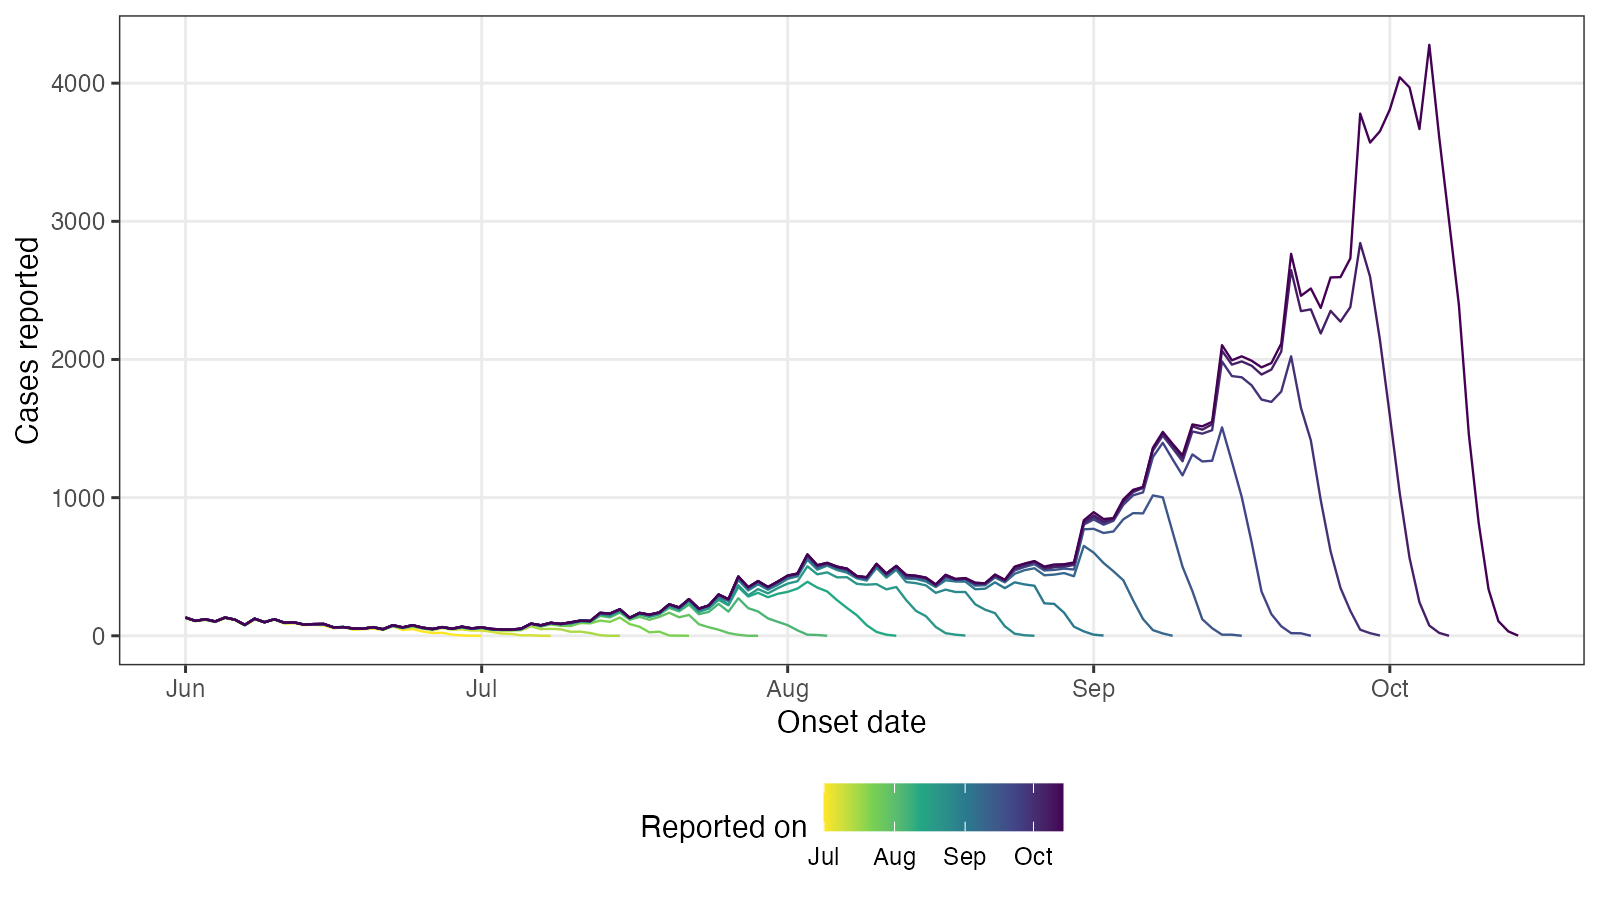
\includegraphics[width=0.85\textwidth]{rivm_snapshots.png}
\caption{Cases by day of symptom onset in the Netherlands, as reported in
every seventh daily file from 1 July to 15 October 2020.}
\label{fig:rivmsnapshots}
\end{figure}

\subsection{Models}

The three models of \S\ref{sec:simulation} were fitted, along with the full
model without batches. $R_t$ was piecewise-constant over periods of seven
onset days and the serial interval was assumed to have mean 5 and standard
deviation 3 days. We took $\Emax=4$ and $\Xmax=30$. Priors were as in
\S\ref{sec:simulation}, except that the priors for the mean and standard
deviation of the reporting delay had means 7 and 5, and the prior for $\eta$
had mean and standard deviation $0.005$. Each fit was a single chain of 800
iterations, of which the first half was discarded. Estimates were compared with
the counts for the same onset days in the file published on 15 October 2020.

\subsection{Results}

\begin{table}[h]
\centering
\begin{tabular}{lccccccc}
\toprule
 & \multicolumn{3}{c}{Latest 14 onset days} & \multicolumn{2}{c}{Reporting delay} & & \\
\cmidrule(lr){2-4}\cmidrule(lr){5-6}
Model & Coverage & Abs.\ error & Bias & Mean & SD & $\rho$ & $\pi$ \\
\midrule
Original & 0.07 & 0.16 & $0.02$ & 8.2 & 5.0 & & \\
Sporadic & 0.14 & 0.16 & $0.02$ & 8.3 & 5.1 & 0.18 & \\
Full without batches & 0.71 & 0.10 & $-0.05$ & 7.1 & 3.7 & 0.059 & 0.042 \\
Full & 0.57 & 0.10 & $-0.03$ & 7.2 & 3.8 & 0.059 & 0.042 \\
\bottomrule
\end{tabular}
\caption{Estimates for the Netherlands made as of 1 September 2020, compared
with the counts known on 15 October 2020. Coverage, absolute error and bias are
as in table~\ref{tab:simulation}. Parameters are posterior medians.}
\label{tab:netherlands}
\end{table}

\begin{figure}[h]
\centering
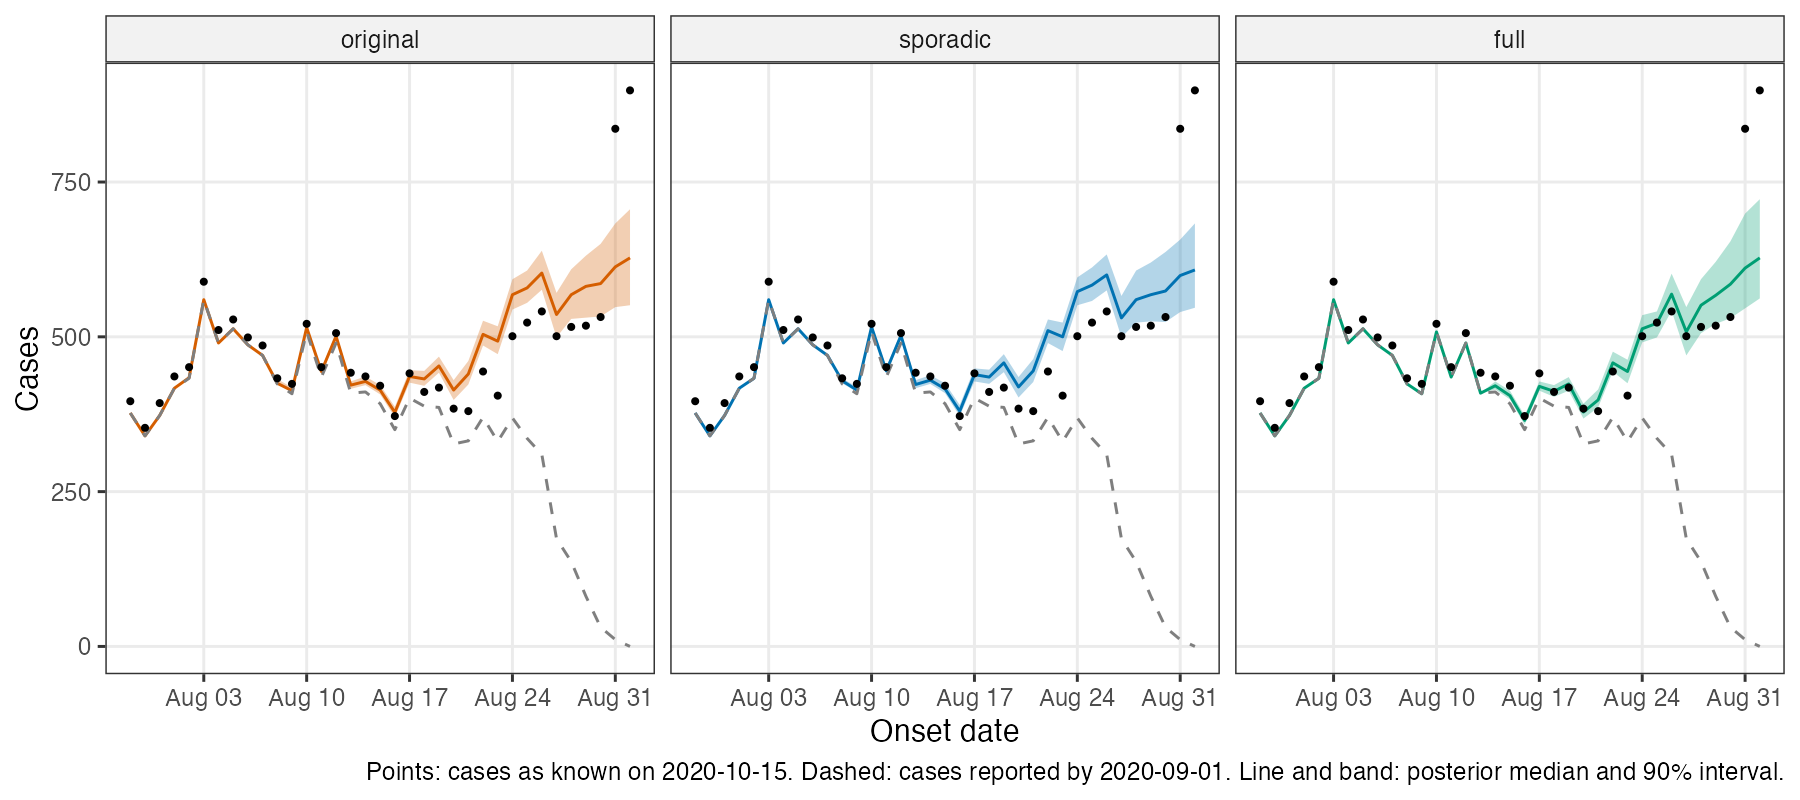
\includegraphics[width=\textwidth]{rivm_nowcast.png}
\caption{Estimates of cases by onset day in the Netherlands made as of
1 September 2020, for three of the models.}
\label{fig:rivmnowcast}
\end{figure}

Table~\ref{tab:netherlands} and figure~\ref{fig:rivmnowcast} show the results.
\begin{itemize}[itemsep=2pt]
\item \emph{Misdating improved the estimates.} With misdating, the absolute
error for the latest 14 onset days fell from 16\% to 10\% and the coverage of
90\% intervals rose from about 0.1 to between 0.6 and 0.7. The misdating
probability was estimated at about 4\% and the estimated reporting delay was
shorter and less variable. Late additions to the count for an onset day, which
the other models must attribute to the tail of the reporting delay, are
instead attributed to corrections.
\item \emph{Batches did not.} The full model performed no better with batches
than without, and took six times as long. It nonetheless placed between two and
five batches of low intensity in every posterior draw, although there is no
large coincident fall in these data. We suspect these to be spurious: a batch
of low intensity is a flexible way of explaining small departures from the
rest of the model.
\item \emph{All models were overconfident.} Coverage was below the nominal 90\%
in every case, and no model anticipated the counts for the final two onset
days, when cases were rising sharply. The renewal model here is Poisson; a
negative binomial renewal model would widen the intervals.
\end{itemize}

\paragraph{Caveats.} This is a single analysis date in a single country. The
serial interval was assumed rather than estimated, and the counts known on
15 October are themselves subject to later revision.

\begin{thebibliography}{1}
\bibitem{bajaj2025}
Bajaj S, Thompson R, Lambert B. 2025
A renewal-equation approach to estimating $R_t$ and infectious disease case
counts in the presence of reporting delays.
\emph{Phil. Trans. R. Soc. A} \textbf{383}, 20240357.
\href{https://doi.org/10.1098/rsta.2024.0357}{doi:10.1098/rsta.2024.0357}
\end{thebibliography}

\end{document}
